%%%%%%%%%%%%%%%%%%%%%%%%%%%%%%%%%%%%%%%%%
% Thin Sectioned Essay
% LaTeX Template
% Version 1.0 (3/8/13)
% This template has been downloaded from:
% http://www.LaTeXTemplates.com
%
% Original Author:
% Nicolas Diaz (nsdiaz@uc.cl) with extensive modifications by:
% Vel (vel@latextemplates.com)
%
% License:
% CC BY-NC-SA 3.0 (http://creativecommons.org/licenses/by-nc-sa/3.0/)
%
%%%%%%%%%%%%%%%%%%%%%%%%%%%%%%%%%%%%%%%%%

%----------------------------------------------------------------------------------------
%	PACKAGES AND OTHER DOCUMENT CONFIGURATIONS
%----------------------------------------------------------------------------------------
\documentclass[12pt]{article} % Font size (can be 10pt, 11pt or 12pt) and paper size (remove a4paper for US letter paper)
\usepackage[protrusion=true,expansion=true]{microtype} % Better typography
\usepackage[left=1in,right=1in,top=1in,bottom=1in]{geometry}
\usepackage{graphicx} % Required for including pictures
\usepackage{wrapfig} % Allows in-line images
%\usepackage{mathpazo} % Use the Palatino font
\usepackage[T1]{fontenc} % Required for accented characters
%\linespread{1.05} % Change line spacing here, Palatino benefits from a slight increase by default
%\usepackage{array}
%\usepackage{booktabs}
%\usepackage{latexsym}
\usepackage{fancyhdr}
\usepackage{lastpage}
\usepackage[pdftex]{hyperref}
\usepackage{tipa}
\usepackage{url}
\usepackage{verbatim}
\hypersetup{
  colorlinks = true,
  urlcolor = black,
  citecolor=black,%
  filecolor=black,%
  linkcolor=black,%
  urlcolor=black     % can put red here to visualize the links
}
%\usepackage{biblatex}

\makeatletter
%\renewcommand\@biblabel[1]{\textbf{#1.}} % Change the square brackets for each bibliography item from '[1]' to '1.'
\renewcommand{\@listI}{\itemsep=0pt} % Reduce the space between items in the itemize and enumerate environments and the bibliography

\renewcommand{\maketitle}{ % Customize the title - do not edit title and author name here, see the TITLE block below
\begin{center} % Right align
{\noindent\@title} % Increase the font size of the title

\vspace{10pt} % Some vertical space between the title and author name

{\noindent\@author}\\\@date

\vspace{10pt} % Some vertical space between the author block and abstract
\end{center}
}


%----------------------------------------------------------------------------------------
%	TITLE
%----------------------------------------------------------------------------------------
%\title{\LARGE{\textbf{Software Engineering Best Practices\\in Biomedical Informatics}\\[.5em]
%}}
%
%\author{\large{Nicholas J. Matiasz}\vspace{.4em}}
%
%\date{\large{2013-10-31}} % Date
%----------------------------------------------------------------------------------------

%----------------------------------------------------------------------------------------
%	HEADER/FOOTER
%----------------------------------------------------------------------------------------
\lhead{}
\chead{}
\rhead{}
\lfoot{BE M227 \textpipe\ Final Exam}
\cfoot{\thepage\ of\ \pageref{LastPage}}
\rfoot{Nicholas J. Matiasz}
\renewcommand{\headrulewidth}{0.4pt}
\renewcommand{\footrulewidth}{0.4pt}
\pagestyle{fancyplain}

%----------------------------------------------------------------------------------------
%	ESSAY BODY
%----------------------------------------------------------------------------------------
\begin{document}

\begin{titlepage}

\newcommand{\HRule}{\rule{\linewidth}{0.5mm}} % Defines a new command for the horizontal lines, change thickness here

\center % Center everything on the page
 
%----------------------------------------------------------------------------------------
%	HEADING SECTIONS
%----------------------------------------------------------------------------------------

\textsc{\Large University of California, Los Angeles}\\[1.5cm] % Name of your university/college
\textsc{\large Medical Imaging Informatics Group}\\[0.5cm] % Major heading such as course name
\textsc{\large BE M227 Final Exam}\\[0.5cm] % Minor heading such as course title

%----------------------------------------------------------------------------------------
%	TITLE SECTION
%----------------------------------------------------------------------------------------
\vspace{20pt}
\HRule \\[0.5cm]
\LARGE{\textbf{Fall 2013 BE M227}}\\[.3cm]
\LARGE{\textbf{Final Exam}}\\
\HRule \\[1.5cm]
 
%----------------------------------------------------------------------------------------
%	AUTHOR SECTION
%----------------------------------------------------------------------------------------

\begin{minipage}{0.4\textwidth}
\begin{flushleft} \large
\emph{Author:}\\
Nicholas J. Matiasz % Your name
\end{flushleft}
\end{minipage}
~
\begin{minipage}{0.4\textwidth}
\begin{flushright} \large
\emph{Instructor:} \\
Prof. Alex Bui % Supervisor's Name
\end{flushright}
\end{minipage}\\[4cm]

% If you don't want a supervisor, uncomment the two lines below and remove the section above
%\Large \emph{Author:}\\
%John \textsc{Smith}\\[3cm] % Your name

%----------------------------------------------------------------------------------------
%	DATE SECTION
%----------------------------------------------------------------------------------------
\begin{minipage}{0.4\textwidth}
\begin{center} \large
\emph{Submitted:} \\
2013-11-26 % Supervisor's Name
\end{center}
\end{minipage}\\[4cm]
%{\large Submitted: 2013-10-30}\\[3cm] % Date, change the \today to a set date if you want to be precise

%----------------------------------------------------------------------------------------
%	LOGO SECTION
%----------------------------------------------------------------------------------------
%\includegraphics{Logo}\\[1cm] % Include a department/university logo - this will require the graphicx package
%----------------------------------------------------------------------------------------
\vfill % Fill the rest of the page with whitespace
\end{titlepage}


\fontsize{12}{28}%22.5, 28
\selectfont
%\thispagestyle{empty}
\tableofcontents
\newpage
\renewcommand\thesection{\arabic{section}}
\renewcommand\thesubsection{\thesection.\alph{subsection}}
\renewcommand\thesubsubsection{\thesubsection.\roman{subsubsection}}

\renewcommand{\arraystretch}{1.5}

\section{Virtual Health Record and Data Integration}

\subsection{Virtual health record and clinical decision support}
Individuals commonly receive medical attention at a variety of institutions throughout their lives.
It follows that their medical records often exist as fragments of information spread across these various locations.
When a patient's medical record exists in a fragmented state, an attending physician must work with only the part of the record to which his institution has access.
Some medical decisions may be suboptimal if they are made on the basis of the information contained in this partial record.
As described in \cite{shortliffe1998}, a virtual health record seeks to synthesize all of this scattered information to achieve a ``distributed but unified summary of all of the health care [patients] have received in their lives.''


An electronic infrastructure that allows separate institutions to share patients' records has the ability to render for physicians a more complete picture of patients' medical histories when care is delivered.
Widely adopted data standards, such as HL7 and DICOM, enable systems at various institutions to share and interpret the same data; these standards are part of initiatives, such as Integrating the Healthcare Enterprise (IHE), that seek greater interoperability across healthcare providers \cite{bui_morioka2010}. The Veterans Health Administration and Kaiser Permanente are two healthcare institutions in the United States that (separately) have fully connected virtual health record systems at all of their locations. Physicians at the VA West Los Angeles Healthcare Center, for example, can access a patient's entire VA medical record, regardless of which other VA locations the patient previously visited.

The ability to access not only a patient's entire medical record but also numerous other records can assist physicians in a variety of ways. Clinical decision support systems---especially those using a Service-Oriented Architecture (SOA)---can use standardized communication protocols (e.g., Simple Object Access Protocol, or SOAP) to pass medical information between organizations \cite{kawamoto2007}. Such decoupled networking tools present low barriers to adoption and facilitate the sharing of medical information, bringing the existing medical infrastructure closer to the ideals proposed in \cite{shortliffe1998}. Additionally, machine-interpretable knowledge bases and machine learning techniques can be used to issue clinically relevant warnings to physicians, including possible adverse drug interactions mined from a patient's record \cite{stead2005}.


\subsection{Data heterogeneity and data integration}
For healthcare systems to implement virtual health records, data from multiple sources need to be aggregated in an intelligible and automated way. A primary difficulty with this task is that different organizations often represent and store their data using different standards, nomenclature, and database architectures. Thus, it is not sufficient simply for a hospital's network to have access to multiple sources of data; an intermediary layer, or \textit{middleware}, is often required to link back end database software with front end information-consuming applications.

These concepts are addressed in detail by Wiederhold \cite{wiederhold1993}, and the challenges he presents in his publication from 1993 remain particularly relevant to the pursuit of healthcare interoperability. Wiederhold discusses many types of data heterogeneity, which are listed in Table \ref{wiederhold}, along with examples. He also suggests that software ``mediators'' process data via four primary functions: abstraction, merging, extrapolation, and caching. The current healthcare environment introduces many complications with respect to these four tasks. The subjective nature of medical interpretation and diagnosis makes the abstraction process very sensitive to errors; the methods used to abstract data for integration may affect any resulting diagnoses. As security is extremely important when handling patient data, extra precaution must be taken when data is merged, extrapolated, or cached. Data that cross firewalls or network boundaries become more susceptible to attacks, and data-processing errors can have not only legal but also medical consequences. The dynamic states of medical knowledge, healthcare legislation, and biomedical technology further complicate any attempts to allow data models (e.g., hierarchies) to be, as Wiederhold suggests, ``adjustable by the user'' \cite{wiederhold1993}. If resources or models are shared across organizations, any adjustment of the representations used for this information will subsequently affect the methods used for integrating this data; all collaborating institutions must be kept up-to-date on such changes.

\begin{table}[h]
\begin{center}
\begin{tabular}{ |l|p{3.33in}| }
\hline
\textbf{Type of data heterogeneity} & \textbf{Example}\\
\hline
heterogeneity of organizational models & mappings across models in networks (e.g., disease models)\\
\hline
heterogeneity in representation & different resolutions (e.g., 5-digit vs. 9-digit zip codes)\\
\hline
heterogeneity of scope &  partially-overlapping categories (e.g., employees vs. personnel vs. payroll vs. health plan)\\
\hline
heterogeneity of abstraction & non-matching atomic data (e.g., locations by zip code vs. locations by town name)\\
\hline
heterogeneity of meaning  & subjective, qualitative attributes (e.g., color)\\
\hline
heterogeneity of temporal validation & different temporal ranges/meanings (e.g., combining an employee's salary, pension, benefits, and bonuses)\\        
\hline
\end{tabular}
\end{center}
\caption{Types of data heterogeneity covered in \cite{wiederhold1993}}
\label{wiederhold}
\end{table}

\section{Peer-to-Peer and Grid Computing}

\subsection{Generations of P2P networks; advantages and disadvantages}
Although numerous examples of peer-to-peer (P2P) networks exist, the evolution of P2P technology can be described as having three generations \cite{bui_taira2010}, which are described below.

\subsubsection{First generation: centralized architecture}
The first generation of P2P networks relied on a centralized architecture in which all nodes communicated with a single index. Such systems combine concepts from both traditional client-server architectures, in which the client and server have different computing roles, and peer-to-peer networks, in which all nodes are approximately equal in functionality \cite{bui_taira2010}. In this first generation of P2P, a requesting node would issue a query to this central index, which kept track of not only what information was currently contained in the network but also which nodes had it. The index would then direct the requesting node to a serving node that could provide the requested data. This strategy had both strengths and weaknesses. Having one central index ensured that all nodes received the same information about the content of the network; however, this concentration of information meant that if the index failed, the entire network was rendered unusable. This architecture also made it difficult for such networks to scale beyond their original size, as the central index becomes a severe bottleneck as the network grows. An example of this first-generation P2P technology was Napster \cite{ratnasamy2002}.

\subsubsection{Second generation: decentralized architecture and distributed hash tables}
The second generation of P2P networks adopted a decentralized architecture and made use of distributed hash tables (DHTs); the five primary commands issued in such networks were \textit{ping}, \textit{pong}, \textit{query}, \textit{queryhit}, and \textit{push}. The decentralized architecture removed the possibility of a central node failure affecting the entire network. This concept was extended further by using DHTs, which save key-value pairs; the information that maps keys to values is decentralized, allowing for more than one node to be able to find data given a key. This approach led to networks that scaled more effectively than first generation designs. The extent to which such a network could scale was constrained by the efficiency of its routing algorithm \cite{ratnasamy2002}. Poor routing algorithms could produce ``query flooding,'' in which unresolved requests for information continue to propagate throughout the network, causing bottlenecks \cite{bui_taira2010}. More efficient routing algorithms can avoid query flooding; instead of a blind search, each query brings the requesting node closer to its target in the key space.
The Chord protocol \cite{stoica2001} and networks based on Gnutella \cite{ratnasamy2002} are examples of the second generation of P2P networks.

\subsubsection{Third generation: anonymization and encryption}
The third generation of P2P networks improved on the advances of the previous two generations and introduced anonymization and encryption.
The fact that this latest generation of P2P is so heavily informed by the previous two has led to frameworks that can be characterized as hybrids of established design concepts \cite{bui_taira2010}.
An example of the third generation of P2P networks is Freenet, which emphasized anonymous file sharing \cite{clarke2001}.

\subsection{Multisite clinical trial with grid and P2P frameworks}
\subsubsection{Cross-Institutional Clinical Translation Research (CICTR)}
The Cross-Institutional Clinical Translational Research (CICTR) project is an example of a project that used grid technologies to enable multisite clinical trials. Three academic institutions---University of Washington, Seattle; University of California, Davis; and University of California, San Francisco---worked together to create a federated query tool that can be used for multisite clinical trial cohort discovery in integrated data repositories (IDR) \cite{anderson2012}.

The three institutions made use of the Informatics for Integrating Biology and the Bedside (i2b2) framework and split this project into three main phases. First, in a move that was perhaps crucial to their success, ``a common technical foundation'' was agreed upon. Second, a ``cohort discovery service'' was tested. Third, the teams managed to ``extend the resolution of cohort data by implementing common queryable mappings to selected medications, laboratory data, and discharge dispositions'' \cite{anderson2012}---a feat that drastically improved the semantic interoperability \cite{decker2000} of the federated data sources.

Although this project's accomplishments were impressive, there were also some limitations. In order to gain IRB approval, the queries had to return aggregated, de-identified, and obscured results. The design process also primarily addressed diabetes-related use cases to facilitate data integration. Nonetheless, CICTR demonstrated the immense amount of information that can be federated when multiple institutions agree on specific technical solutions and implement grid computing techniques.

\subsubsection{The caGrid framework}
The caGrid framework is an open-source, service-oriented architecture (SOA) that is based on the Globus architecture \cite{foster1999}. It was designed to enable greater collaboration across multiple teams engaged in cancer research \cite{oster2008}. The framework achieved this using a multi-tier (n-tier) architecture that provided various web services, including enterprise vocabulary services (EVS), cancer bioinformatics infrastructure objects (caBIO), and cancer data standards repositories (caDSR) \cite{bui_taira2010}. Like other successful projects emphasizing interoperability, a standard language---in this case, the Business Process Execution Language (BPEL)---was used to execute web service requests in the grid environment; multiple markup languages (e.g., Security Assertion Markup Language, Extensible Access Control Markup Language, etc.) were also implemented \cite{oster2008}.

\subsubsection{Shared Pathology Informatics Network (SPIN)}
The Shared Pathology Informatics Network (SPIN) \cite{mcmurry2007} is a third example of P2P and grid technologies being used to facilitate multisite trials. Multiple institutions can join the SPIN network as nodes within a P2P network, and the level of access afforded by each peer is commensurate with the IRB approval granted by each participating institution. With this architecture, the security of each data resource can be monitored appropriately by the organization responsible for it, and the P2P architecture scales readily.


\section{Centralized vs. Distributed Computing}
\subsection{Comparison of the two architectures}
The following sections compare centralized and distributed architectures. See Figures \ref{centralized} and \ref{distributed} for examples of these two architectures realized via client-server relationships.

\begin{figure}[h]
\centering
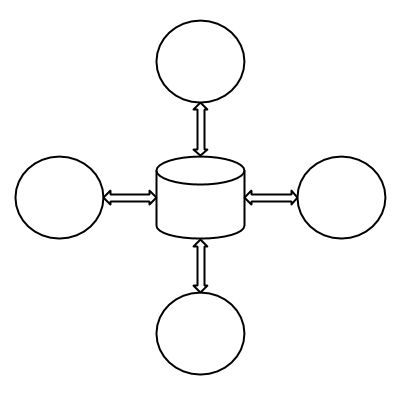
\includegraphics[scale=.75]{./images/centralized.png}
\caption{A centralized client-server architecture.}
\label{centralized}
\end{figure}

\begin{figure}[h]
\centering
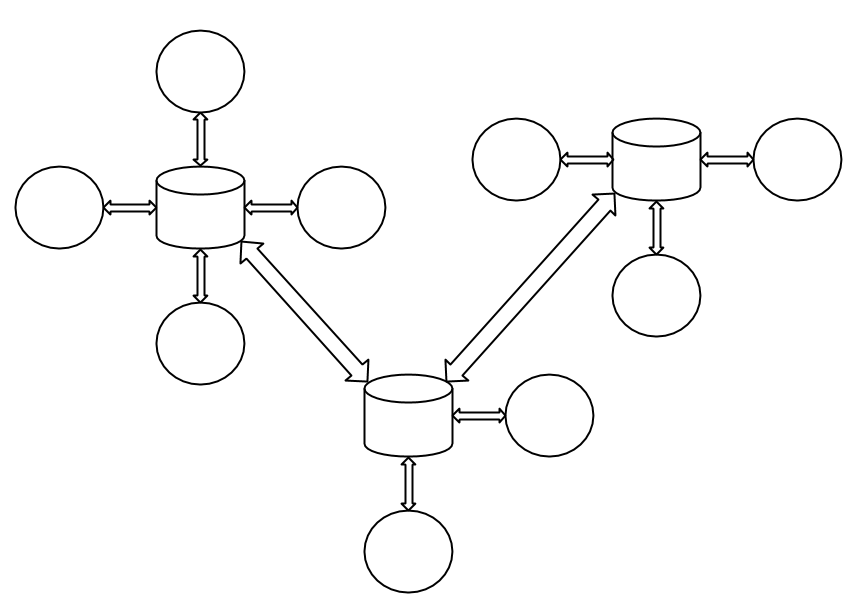
\includegraphics[scale=.75]{./images/distributed.png}
\caption{A distributed client-server architecture.}
\label{distributed}
\end{figure}




\subsubsection{Security and authentication}
For the simple reason that distributed architectures invite implementations involving highly connected networks, these systems usually come with greater security vulnerabilities. A centralized system can keep a single record of the credentials of all users, modules, etc. that comprise the network; however, a distributed system must often keep multiple copies of this information, which complicates the enforcement of security protocols.
\subsubsection{Data replication}
Centralized architectures rely less on data replication than distributed architectures because all of the information that is pertinent to the system with a centralized architecture is stored in a single, central node or server. By definition, distributed architectures require multiple copies of information (or other resources) so that the entire network does not rely on a single node or layer in the network to perform a function.
\subsubsection{Data updating}
The maintenance of centralized systems is often more straightforward than that of distributed systems. This is due to the fact that distributed systems often maintain multiple copies of a information and resources. For consistency, distributed systems must find a way to update all of these instances, without becoming vulnerable to the consequences of asynchronous updates.
\subsubsection{Processing throughput and bottlenecks}
Centralized systems usually experience a greater number and severity of bottlenecks; their reliance on a single resource also makes them more likely to fail. For similar reasons, centralized architectures are also less extensible.

\section{Design an EHR} 
\subsection{A proposal for a national EHR}
The following sections propose a design for a national infrastructure for an electronic health record (EHR) that could contain an entire lifetime worth of patient data.
\subsubsection{A model for medical record information}
Although it is arguably a data standard, the use of Extensible Markup Language (XML), or, in the very least, some form of markup language, is likely going to be essential for national interoperability efforts. The value of this approach is indicated by the large number of medical informatics research projects (e.g., \cite{mcmurry2007, oster2008, weber2009}) that have used XML in their designs.
A universal and immutable language and/or machine-interpretable EHR definition is unlikely ever to manifest in a single, discrete design effort; even if the entire nation could agree on such a scheme, its evolution would result in massive, if not infeasible, maintenance efforts and would require very restrictive top-down management. The use of a markup language is ideal in this case for two reasons. First, instead of a rigid data standard that may be costly to adopt, it is more of a strategy---a general technical solution---that can be implemented slowly and with greater precision over time. Second, XML is inherently extensible, so it is a perfect candidate for the communication of medical information, whose vocabulary is constantly evolving. This idea is discussed at length by Decker, et al. \cite{decker2000}, who argue that the use of XML is a key to achieving semantic interoperability. If, for example, a new medical term comes into use, XML can accommodate the inclusion of this term in subsequent medical records without completely dismantling the hierarchies, ontologies, and other models already in place.

Regarding higher-level EHR designs, there has been much debate about optimal EHR solutions, with no clear winner in sight. Nonetheless, concepts such as scalability, extensibility, and loose coupling of modules appear frequently in the literature, as these characteristics are highly desirable in the context of national healthcare interoperability.  In 2009, Blobel and Pharow \cite{blobel2009} conducted an analysis of existing EHR models, and concluded that regardless of which EHR implementation is adopted, adherence to the Generic Component Model (GCM) is essential to achieve scalability and loosely coupled modules for communication. The HL7 Clinical Document Architecture (CDA), despite its limitations, is an attractive option given its minimal document requirement of XML tags for only a header and a body \cite{dolin2006}. A modest implementation of this standard is therefore within reach of institutions lacking significant IT expertise.

\subsubsection{A method for secure communication of medical information}
In the absence of top-down governmental control over all medical information, a single, centralized mechanism for storing medical information should not exist (see Section \ref{ehr_storage} for further discussion on this point). Therefore, if healthcare providers are to be responsible for storing the medical data that is generated at their facilities, the means for communicating these findings, like the storage strategy, will need to be highly distributed. The web-services-based grid architecture used by caGrid \cite{oster2008} provides a nice example of the kind of distributed framework that will be necessary for national interoperability. The use of web services will motivate each member of the network to articulate the precise application programming interface (API) that is required for data exchange. APIs are advantageous in this context for two reasons: (1) they commonly use markup languages (e.g., XML, JSON) to format information, and (2) they are extensible, so that functionality can be added incrementally as participating providers improve their data-sharing abilities.

\subsubsection{A network topology for linking health institutions}
The network topology for a national EHR infrastructure should accommodate incremental growth of the network, and should not implicitly or explicitly enforce any hierarchies among members of the network; in other words, all healthcare organizations should be able to participate without falling victim to undue technological subservience. This requirement motivates the selection of a P2P architecture for a national EHR solution. Although enforcing a slight hierarchy with its use of supernodes, the design presented in \cite{mcmurry2007} illustrates just how powerful a distributed, loosely coupled P2P network can be for facilitating the communication of medical data. The P2P implementation would have to eschew the anonymization abilities afforded by the third generation of P2P so that requests for information sent over the network could be evaluated with respect to the credentials of the institution or individual that initiated the request.

Although P2P networks have historically been used for less computationally intensive applications, such as file sharing, Foster and Iamnitchi \cite{foster2003} argue that P2P and grid computing are not mutually exclusive methods. Furthermore, they suggest that hybrid techniques will eventually harness both the extensibility of P2P networks and the immense computing power of grid networks.

\subsubsection{A method for secure storage of medical information} \label{ehr_storage}
The proposed EHR implementation requires a P2P architecture in which medical data is stored at the location where it is obtained.
Rather than trying to enforce a single, universal security policy in all of the diverse medical contexts that exist, each institution is left to choose a technical strategy for satisfying the security requirements that are imposed by law (e.g., HIPAA). By communicating medical information via web service APIs, healthcare organizations would have specific control over the type of information that crosses its network boundaries. To further promote the technological cooperation motivated by the P2P architecture, public-key encryption \cite{barrows1996} would be used for all storage (and subsequent communication) of medical information.

\subsubsection{A method for searching for patients' medical information}
Admittedly, if organizations are to share medical information, any protocol that would entirely eliminate the chance of a security breach would likely also render the system useless to physicians. Some level of trust needs to be assumed for a national EHR solution to be effective in existing clinical workflows \cite{murphy2011}. Therefore, the ability to search a national resource of health data would require that providers maintain an appreciable level of transparency for their data resources. Given that a patient's medical data would always be stored at the location where it was obtained, knowledge of where a patient has previously received medical attention would inform which institution's web services should be queried for that patient's data. Such information might not always be available, but implementing a practice of recording patients' ``geographical medical history,'' despite sacrificing some privacy, would greatly facilitate the search process.

\subsection{Challenges and solutions for adoption and implementation}
If top-down government legislation cannot be used to direct the course of healthcare's evolution, the technological barriers to interoperability must be lowered as much as possible, so that organizations with less robust budgets and IT expertise can keep pace.
If healthcare does not implement a pay-for-performance scheme, economic incentives for achieving inter-institutional interoperability are likely to exist solely as positive externalities, which, in a free market, are unlikely to be sufficiently motivating.
Therefore, any effort to implement a national infrastructure for an EHR that cannot rely on mandating data standards and national-level identifiers must instead use a highly iterative process that promotes extensible and adaptable solutions.

These challenges further highlight the value of adopting a web-services-based approach to national healthcare interoperability. The ability of APIs to be implemented incrementally over time would minimize technological barriers to joining a national EHR network. With institutions speaking the same programmatic language---at least on the level of APIs, if not also on the level of markup languages and document specifications (e.g., HL7)---healthcare organizations would enjoy increasing connectivity and access to resources. Like the implementation reported in \cite{mcmurry2007}, each organization would still control the security protocols for its data, and legal concerns surrounding this unprecedented level of connectivity would be attenuated.

%----------------------------------------------------------------------------------------
%	BIBLIOGRAPHY
%----------------------------------------------------------------------------------------
\newpage
\bibliographystyle{plain}
\bibliography{m227_final_exam}
%----------------------------------------------------------------------------------------

\end{document}